\subsection{РЕЗУЛЬТАТЫ МОДЕЛИРОВАНИЯ}

На языке программирования C++ была реализована столбчатая модель ГЭЦ, которая позволяет рассчитывать ИП при любом задании токов источников и проводимости воздуха. Так как параметризация источников, описанная в разделе \ref{sec:sources}, имеет ясный физический смысл, то ниже всюду будет использоваться именно она.

ИП и электрическое поле в регионах хорошей погоды имеют замечательную особенность --- устойчивую кривую суточной вариации. Такую кривую называют кривой Карнеги \cite{Harrison_2012} (см. рис. \ref{fig:carnegie_curve}). Ее форма объясняется динамикой глобальных грозовых центров, происходящей на масштабах суток \cite{Ilin_et_al_2020}. Кривая Карнеги служит хорошим объектом для проверки адекватности работы реализованной столбчатой модели ГЭЦ. 

\begin{figure}  
    \centering
    \begin{subfigure}[t]{.49\textwidth}
		\centering
		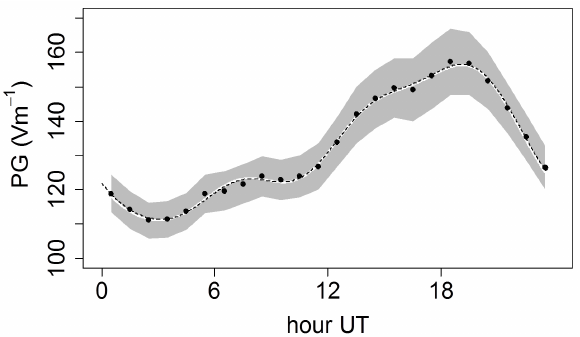
\includegraphics[width=\linewidth]{figures/carnegie_curve.png}
		\caption{}
		\label{fig:carnegie_curve}  
    \end{subfigure}
    \hfill
    \begin{subfigure}[t]{.49\textwidth}
		\centering
		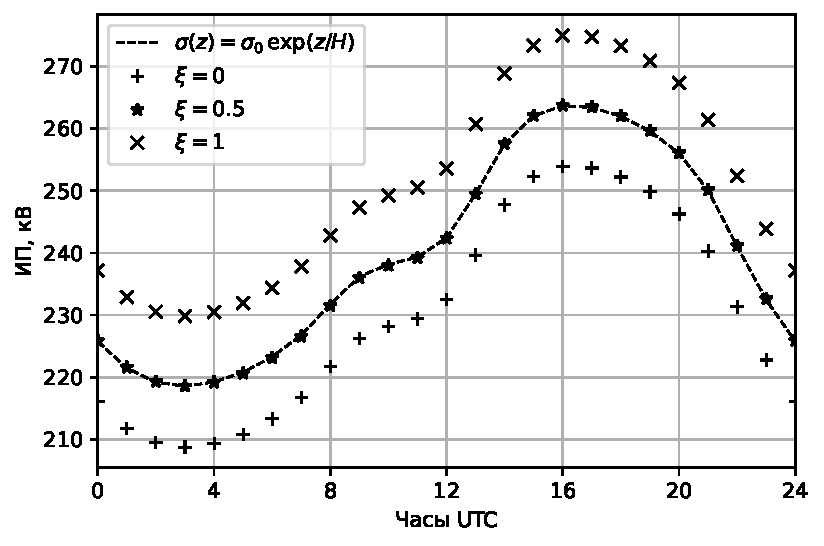
\includegraphics[width=\linewidth]{figures/ip_differences.pdf}
		\caption{}
		\label{fig:ip_differences}  
     \end{subfigure}
     \caption{(a): Черные точки изображают вариацию приповерхностного градиента потенциала электрического поля (potential gradient, PG) по часам всемирного времени (UTC), измеренную на корабле Карнеги в 1920-ые годы. Серая область вокруг точек обозначает плюс и минус одну стандартную ошибку среднего. Черная пунктирная и белая линии обозначают различные гладкие аппроксимации экспериментальных данных. Взято из \cite[Рис. 6a]{Harrison_2012} (b): Пунктирной линией обозначена кривая суточной вариации ИП, полученная при усреднении результатов моделирования ИП с экспоненциальной проводимостью (см. раздел \ref{sec:exp_sigma}) за каждый третий день 2016 года. Суточные вариации ИП, получаемые при использовании параметризации проводимости, описанной в разделе \ref{sec:complicated_sigma}, отмечены точечными маркерами: маркер плюс отвечает моделированию при параметре $\xi$, описывающем солнечную активность, равном 0; маркер звездочка --- при $\xi = 0.5$; маркер крест --- при $\xi = 1$.}
	\label{fig:variations-1}  
\end{figure}

Параметризация источников, описанная в разделе \ref{sec:sources}, требует задания таких параметров, как высоты изотерм, осадки, запасенная влага и CAPE, которые берутся из результатов воспроизведения атмосферной динамики. Для этих целей использовалась метеорологическая модель WRF, позволившая получить требуемые для расчета ИП параметры в виде 24-часового набора данных за каждый третий день 2016 года на широтно-долготной сетке 1\textdegree\texttimes1\textdegree. На основе данных, полученных из модели WRF, рассчитывался ИП. В результате таких расчетов получался 24-часовой набор значений ИП для каждого третьего дня 2016 года.

Было произведено несколько серий расчетов ИП. В различных сериях расчетов использовались разные параметризации проводимости: в одном из расчетов была задействована параметризация проводимости, описанная в разделе \ref{sec:exp_sigma}, в прочих расчетах использовалась более сложная параметризация проводимости, которой был посвящен раздел \ref{sec:complicated_sigma}), с различными параметрами солнечной активности $\xi$. 

Результаты расчетов ИП усреднялись по всем моделируемым дням, чтобы получить кривую суточной вариации ИП (даже моделируемый ИП крайне изменчив на масштабах суток, поэтому для обнаружения характерной кривой суточной вариации необходимо усреднять данные по достаточно долгому периоду времени). В итоге были получены кривые суточной вариации ИП, изображенные на рис. \ref{fig:ip_differences}.

Из анализа полученных кривых удается сделать три вывода. Первый состоит в том, что разработанная модель ГЭЦ позволяет получать кривую суточной вариации ИП, близкую к оригинальной кривой Карнеги (как видно из сравнения рис. \ref{fig:ip_differences} с рис. \ref{fig:carnegie_curve}), что подтверждает верность реализации столбчатой модели ГЭЦ. Второй вывод заключается в том, что форма кривой суточной вариации ИП, получающаяся при моделировании с экспоненциальной проводимостью, совпадает с формой кривой суточной вариации, которая получается при моделировании с учетом более реалистичной проводимости (см. рис. \ref{fig:ip_differences}), то есть кривые имеют максимумы и минимумы в одни и те же часы UTC. В качестве третьего вывода следует отметить, что учет более реалистичной проводимости приводит к повышению ИП примерно на $10\, \textnormal{кВ}$ в фазу максимума солнечной активности и к понижению примерно на те же $10\, \textnormal{кВ}$ в фазу минимума солнечной активности по сравнению со значениями ИП, получаемыми при моделировании с экспоненциальной проводимостью.